\documentclass{standalone}

\usepackage{xcolor}

\definecolor{myblue}{HTML}{377EB8}
\definecolor{myred}{HTML}{E41A1C}

\usepackage{tikz}
\usepackage{pgfplots}
\pgfplotsset{compat=newest}

\usepackage{lmodern}
\SetSymbolFont{letters}{bold}{OML}{cmbr}{bx}{it}
\renewcommand{\familydefault}{\sfdefault}

\usepackage{sansmathfonts}

\begin{document}
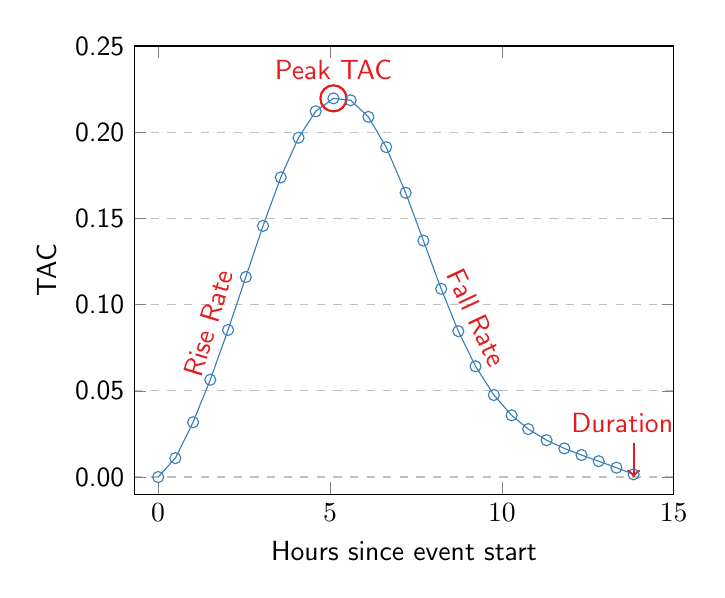
\begin{tikzpicture}
	\begin{axis}[
			xlabel={Hours since event start},
			ylabel={TAC},
			xmin=-0.70, xmax=15,
			ymin=-0.01, ymax=.25,
			xtick={0,5,10,15},
			ytick={0,0.05, 0.10,0.15,0.20,0.25},
			yticklabels={0.00,0.05, 0.10,0.15,0.20,0.25},
			ymajorgrids=true,
			grid style=dashed,
		]
						
		\addplot[
			color=myblue,
			mark=o,
		]
		coordinates {
			(0, 0)
			(0.5, 0.010956182)
			(1.016666667, 0.031769215)
			(1.516666667, 0.056414075)
			(2.033333334, 0.08528632)
			(2.55, 0.116005901)
			(3.05, 0.145641834)
			(3.566666667, 0.173785905)
			(4.083333334, 0.196795234)
			(4.583333334, 0.212115906)
			(5.1, 0.219609466)
			(5.6, 0.218491637)
			(6.116666667, 0.208877435)
			(6.633333334, 0.191321648)
			(7.2, 0.164858595)
			(7.716666667, 0.137092347)
			(8.233333334, 0.109137118)
			(8.733333334, 0.084597977)
			(9.233333334, 0.064228751)
			(9.766666667, 0.047560616)
			(10.28333333, 0.035802902)
			(10.76666667, 0.027816521)
			(11.3, 0.021369497)
			(11.81666667, 0.01661389)
			(12.31666667, 0.01275028)
			(12.81666667, 0.009167184)
			(13.33333333, 0.005421836)
			(13.83333333, 0.001547828)    
		};
		\node[above,myred] at (5.1,0.225) {Peak TAC};
		\node[myred,draw,circle,thick] at (5.1,0.219609466) {};
		\node[left,myred,rotate=73] at (2,0.125) {Rise Rate};
		\node[right,myred,rotate=-65] at (8.5,0.125) {Fall Rate};
		% \node[right,myred] at (4.3,0.125) {AUC};
		\node[above,myred] at (13.5,0.02) {Duration};
		\draw[myred,->,thick] (13.83333333,0.02) -- (13.83333333,0);
	\end{axis}
\end{tikzpicture}
\end{document}
